\documentclass[cs4size,a4paper]{ctexart}   
%===数学符号公式===
\usepackage{amsmath}    					% AMS LaTeX宏包
\usepackage[style=1]{mdframed}
\usepackage{amsthm}
\usepackage{amssymb}
\usepackage{bm}                      	% 数学公式中的黑斜体
\usepackage{bbm}
\usepackage{amsfonts}
\usepackage{mathrsfs}                	% 英文花体字 体
\usepackage{bbding,manfnt}    			% 一些图标,如 \dbend
\usepackage{lettrine}                	% 首字下沉,命令\lettrine
\def\attention{\lettrine[lines=2,lraise=0,nindent=0em]{\large\textdbend\hspace{1mm}}{}}
\usepackage{longtable}
\usepackage{enumerate}
\usepackage[toc,page]{appendix}
\usepackage{geometry}         			% 页边距调整
\geometry{top=3.0cm,bottom=2.7cm,left=2.5cm,right=2.5cm}
\usepackage[colorinlistoftodos,prependcaption,textsize=small]{todonotes}
%===公式按章编号===
\numberwithin{equation}{section}
\numberwithin{table}{section}
\numberwithin{figure}{section}
%===基本格式预置===
\usepackage{fancyhdr}
\pagestyle{fancy}
\fancyhf{}  
\fancyhead[C]{\zihao{5}  \kaishu 矩阵的谱半径}
\fancyfoot[C]{~\zihao{5} \thepage~}
\renewcommand{\headrulewidth}{0.75pt} 
\CTEXsetup[format={\centering\bfseries\zihao{-2}},name={第, 章}]{section}
\CTEXsetup[nameformat={\bfseries\zihao{3}}]{subsection}
\CTEXsetup[nameformat={\bfseries\zihao{4}}]{subsubsection}
%===图形支持宏包===
\usepackage{graphicx}        			% 嵌入png图像
\usepackage{subfigure}
\usepackage{float}
\graphicspath{{figure/}}
\usepackage{color,xcolor}     			% 支持彩色文本、底色、文本框等
\usepackage[colorlinks,linkcolor=blue,anchorcolor=blue,citecolor=blue]{hyperref}
%\usepackage{caption}
\usepackage[ruled,linesnumbered]{algorithm2e}
%\captionsetup{figurewithin=section}
%===源码和流程图===
\usepackage{listings,fontspec}         	% 粘贴源代码
\newfontfamily\monaco{Monaco}
\definecolor{mygreen}{rgb}{0,0.6,0}
\definecolor{mygray}{rgb}{0.5,0.5,0.5}
\definecolor{mymauve}{rgb}{0.58,0,0.82}
\lstset{ %
backgroundcolor=\color{white},   		% choose the background color
basicstyle=\footnotesize\monaco,       % size of fonts used for the code
columns=fullflexible,
breaklines=true,                 		% automatic line breaking only at whitespace
captionpos=b,                    		% sets the caption-position to bottom
tabsize=4,
commentstyle=\color{mygreen}\monaco,   % comment style
escapeinside={\%*}{*)},          		% if you want to add LaTeX within your code
keywordstyle=\color{blue}\monaco,      % keyword style
stringstyle=\color{mymauve}\monaco,    % string literal style
frame=single,
rulesepcolor=\color{red!20!green!20!blue!20},
% identifierstyle=\color{red},
language=python,
}
%===颜色===
\usepackage{color,xcolor}
\definecolor{dkgreen}{rgb}{0,0.6,0}
\definecolor{gray}{rgb}{0.5,0.5,0.5}
\definecolor{mauve}{rgb}{0.58,0,0.82}
 \usepackage{xcolor}
 \lstset{
  %行号
   numbers=left,
   %背景框
   framexleftmargin=8mm,
   frame=none,
   %背景色
   %backgroundcolor=\color[rgb]{1,1,0.76},
   backgroundcolor=\color[RGB]{245,245,244},
   %样式
   keywordstyle=\bf\color{blue},
   identifierstyle=\bf,
   numberstyle=\color[RGB]{0,192,192},
   commentstyle=\it\color[RGB]{0,96,96},
   stringstyle=\rmfamily\slshape\color[RGB]{128,0,0},
   %显示空格
   showstringspaces=false
 }

%--------------------
\hypersetup{hidelinks}
\usepackage{booktabs}  
\usepackage{shorttoc}
\usepackage{tabu,tikz}
\usepackage{float}
\usepackage{multirow}

\tabcolsep=1ex
\tabulinesep=\tabcolsep
\newlength\tikzboxwidth
\newlength\tikzboxheight
\newcommand\tikzbox[1]{%
        \settowidth\tikzboxwidth{#1}%
        \settoheight\tikzboxheight{#1}%
        \begin{tikzpicture}
        \path[use as bounding box]
                (-0.5\tikzboxwidth,-0.5\tikzboxheight)rectangle
                (0.5\tikzboxwidth,0.5\tikzboxheight);
        \node[inner sep=\tabcolsep+0.5\arrayrulewidth,line width=0.5mm,draw=black]
                at(0,0){#1};
        \end{tikzpicture}%
        }
\makeatletter
\def\hlinew#1{%
  \noalign{\ifnum0=`}\fi\hrule \@height #1 \futurelet
   \reserved@a\@xhline}
   
\usepackage{CJK}
\usepackage{ifthen}
\newcommand{\HRule}{\rule{\linewidth}{0.5mm}}
\newcommand{\tabincell}[2]{\begin{tabular}{@{}#1@{}}#2\end{tabular}}%
%===使得公式随章节自动编号===
\makeatletter
\@addtoreset{equation}{section}
\makeatother
\renewcommand{\theequation}{\arabic{section}.\arabic{equation}}
%-------------------------
\usepackage{pythonhighlight}
\usepackage{tikz}                    
\usepackage{tikz-3dplot}
\usetikzlibrary{shapes,arrows,positioning}
%===正文开始===
\begin{document}
%===定理类环境定义===
\newtheorem{example}{例}              	% 整体编号
\newtheorem{algorithem}{算法}	
\newtheorem{theorem}{定理}            	% 按section编号
\newtheorem{definition}{定义}
\newtheorem{axiom}{公理}
\newtheorem{property}{性质}
\newtheorem{proposition}{命题}
\newtheorem{lemma}{引理}
\newtheorem{corollary}{推论}
\newtheorem{remark}{注解}
\newtheorem{condition}{条件}
\newtheorem{conclusion}{结论}
\newtheorem{assumption}{假设}
%===重定义===
\renewcommand{\contentsname}{目录}     
\renewcommand{\abstractname}{摘要} 
\renewcommand{\refname}{参考文献}     
\renewcommand{\indexname}{索引}
\renewcommand{\figurename}{图}
\renewcommand{\tablename}{表}
\renewcommand{\appendixname}{附录}
\renewcommand{\proofname}{证明}
%\renewcommand{\algorithm}{算法} 
\renewcommand\emph[1]{\textcolor{red}{\textbf{#1}}}
%===封皮和前言===
\begin{titlepage}
\begin{center}
% Upper part of the page

\includegraphics[width=0.15\textwidth]{logo}\\[1cm]    
\textsc{\Large Beijing University of Chemical Technology}\\[1.0cm]
\textsc{\Large Course Homeworks}\\[0.5cm]
% Title
\HRule \\[0.8cm]
{\huge \bfseries 矩阵的谱半径}\\[0.4cm]
\HRule \\[0.7cm]
% Author
\textsc{计科1703 张俊峰 2017040330}
\tableofcontents 
\vfill
% Bottom of the page
{创建日期:2019年11月19日}\\
{更新日期:\today}
\end{center}
\end{titlepage}
\pagestyle{plain}
\pagenumbering{Roman}
\thispagestyle{empty}
%===正文===
\pagestyle{fancy}
\pagenumbering{arabic}

%===第一章===
\section{矩阵的谱半径}
\subsection{简介}
设$ A $是$ n × n $矩阵~,~$ \lambda_1,...,\lambda_n $是其特征值~,~则A的谱半径$ \rho\left(A\right)=\max\left\{\left|\rho_1\right|,...,\left|\rho_n\right|\right\} .$

\begin{enumerate}[\quad\quad(1)]
\item 矩阵的谱半径等于矩阵的特征值绝对值的最大值。
\item 在数学中,矩阵的谱半径是指其特征值绝对值集合的上确界。
\end{enumerate}


\subsection{理论分析}


\begin{theorem}
\label{rotM}
设$ A \in R^{n \times n} $为$ n $ 阶方阵~,~则对任意矩阵范数$ \left|\left|\cdot\right|\right| $都有$ \rho\left(A\right)\leq\left|\left|\cdot\right|\right| $~.~
\end{theorem}

\begin{theorem}
\label{rotM}
若$ A $为$ n $ 阶正规矩阵~,~则$ \rho\left(A\right)\leq\left|\left|A\right|\right|_2 $~.~
\end{theorem}


\begin{proof}
因$ A $是正规矩阵~,~故存在幺正矩阵$ P $~,~使得
\begin{align}
\label{P^HAP}
  P^HAP=\begin{bmatrix} \lambda_1&~ ~ &~ ~ \\
				   ~ ~&~...~&~ ~\\
				   ~ ~&~ ~&\lambda_n
\end{bmatrix} 
\end{align}
\end{proof}

~ ~由此可得:
\begin{align}
\label{P^HA^HP}
  P^HA^HP=\begin{bmatrix}\bar{\lambda_1}&~ ~ &~ ~ \\
				~ ~&~...~&~ ~\\
				~ ~&~ ~&\bar{\lambda_n}
\end{bmatrix}
\end{align}

~   ~从而:
\begin{align}
\label{P^HA^HAP}
  P^HA^HAP=\begin{bmatrix}\left|\lambda_1\right|^2&~ ~ &~ ~ \\
				~ ~&~...~&~ ~\\
				~ ~&~ ~&\left|\lambda_n\right|^2
\end{bmatrix}
\end{align}

~   ~又显然有:
\begin{displaymath}
\lambda_AH_A ~=~ \max\left\{\left|\lambda_1\right|^2 ~,~ \left|\lambda_2\right|^2 ~,...,~ \left|\lambda_n\right|^2\right\} ~=~ \left|\lambda_t\right|^2.
\end{displaymath}

~  ~这里$ t $是$ \left\{1, 2, ...,n\right\} $中的某一值,因此有:
\begin{displaymath}
\left|\left|A\right|\right|_2 ~=~ \sqrt{\lambda_AH_A} ~=~ \left|\lambda_t\right|.
\end{displaymath}

~  ~又因为:
\begin{displaymath}
\rho\left(A\right)~=~\max\left\{\left|\lambda_1\right| ~,~ \left|\lambda_2\right| ~,...,~ \left|\lambda_n\right|\right\} ~=~ \left|\lambda_t\right|
\end{displaymath}

~  ~所以,可以证明:
\begin{displaymath}
\rho\left(A\right)\leq\left|\left|A\right|\right|_2
\end{displaymath}

\subsection{算法描述}

\begin{algorithm}[H]
\caption{算法}\label{algorithm}
\KwIn{要进行计算你的矩阵的行与列,并且按照行的顺序依次输入矩阵元素;}
\KwOut{该矩阵的所有特征值和矩阵的谱半径(绝对值最大的特征值);}
输入矩阵的行与列以及矩阵内的元素;

$ bool~ ~InitMatrix(Matrix~ ~*matrix,~ ~int~ ~row,~ ~int~ ~column) $

定义一个结构体,用来表示二维矩阵;

$typedef~ ~struct $

$ \{ $

$     ~   ~int~ ~row; $

$     ~   ~int~ ~column; $

$     ~   ~double~ ~*data; $

$\}Matrix; $

使用QR分解求矩阵特征值

$ for~ ~k~=~0 \rightarrow NUM $

$ \{  $

$    QR(temp,~ ~temp_Q,~ ~temp_R); $

$	MatrixMulMatrix(temp,~ ~temp_R,~ ~temp_Q); $ 分解后两个矩阵相乘

$ \} $

获取特征值,将特征值存储在 $eValue$中

$ for~ ~k~=~0 \rightarrow temp.column$

$\{$

$eValue.data[k] ~=~ temp.data[k~*~temp.column ~+~ k];$

$result[k] ~=~ fabs(temp.data[k ~*~ temp.column ~+~ k]);$

$\}$

输出特征值以及矩阵的谱半径

$ float~ ~maxn~ =~ -1 $

$ for~ ~k~=~0 \rightarrow temp.column$

$\{$

$ if~ ~(result[k] ~>~ maxn)$

$maxn ~=~ result[k];$

$\}$

$ PrintMatrix(eValue); $
 
$printf $ 矩阵的谱半径(即特征值绝对值最大)为: $ maxn;$
\end{algorithm} 


\subsection{实例分析}

\begin{figure}[H]
\small
\centering
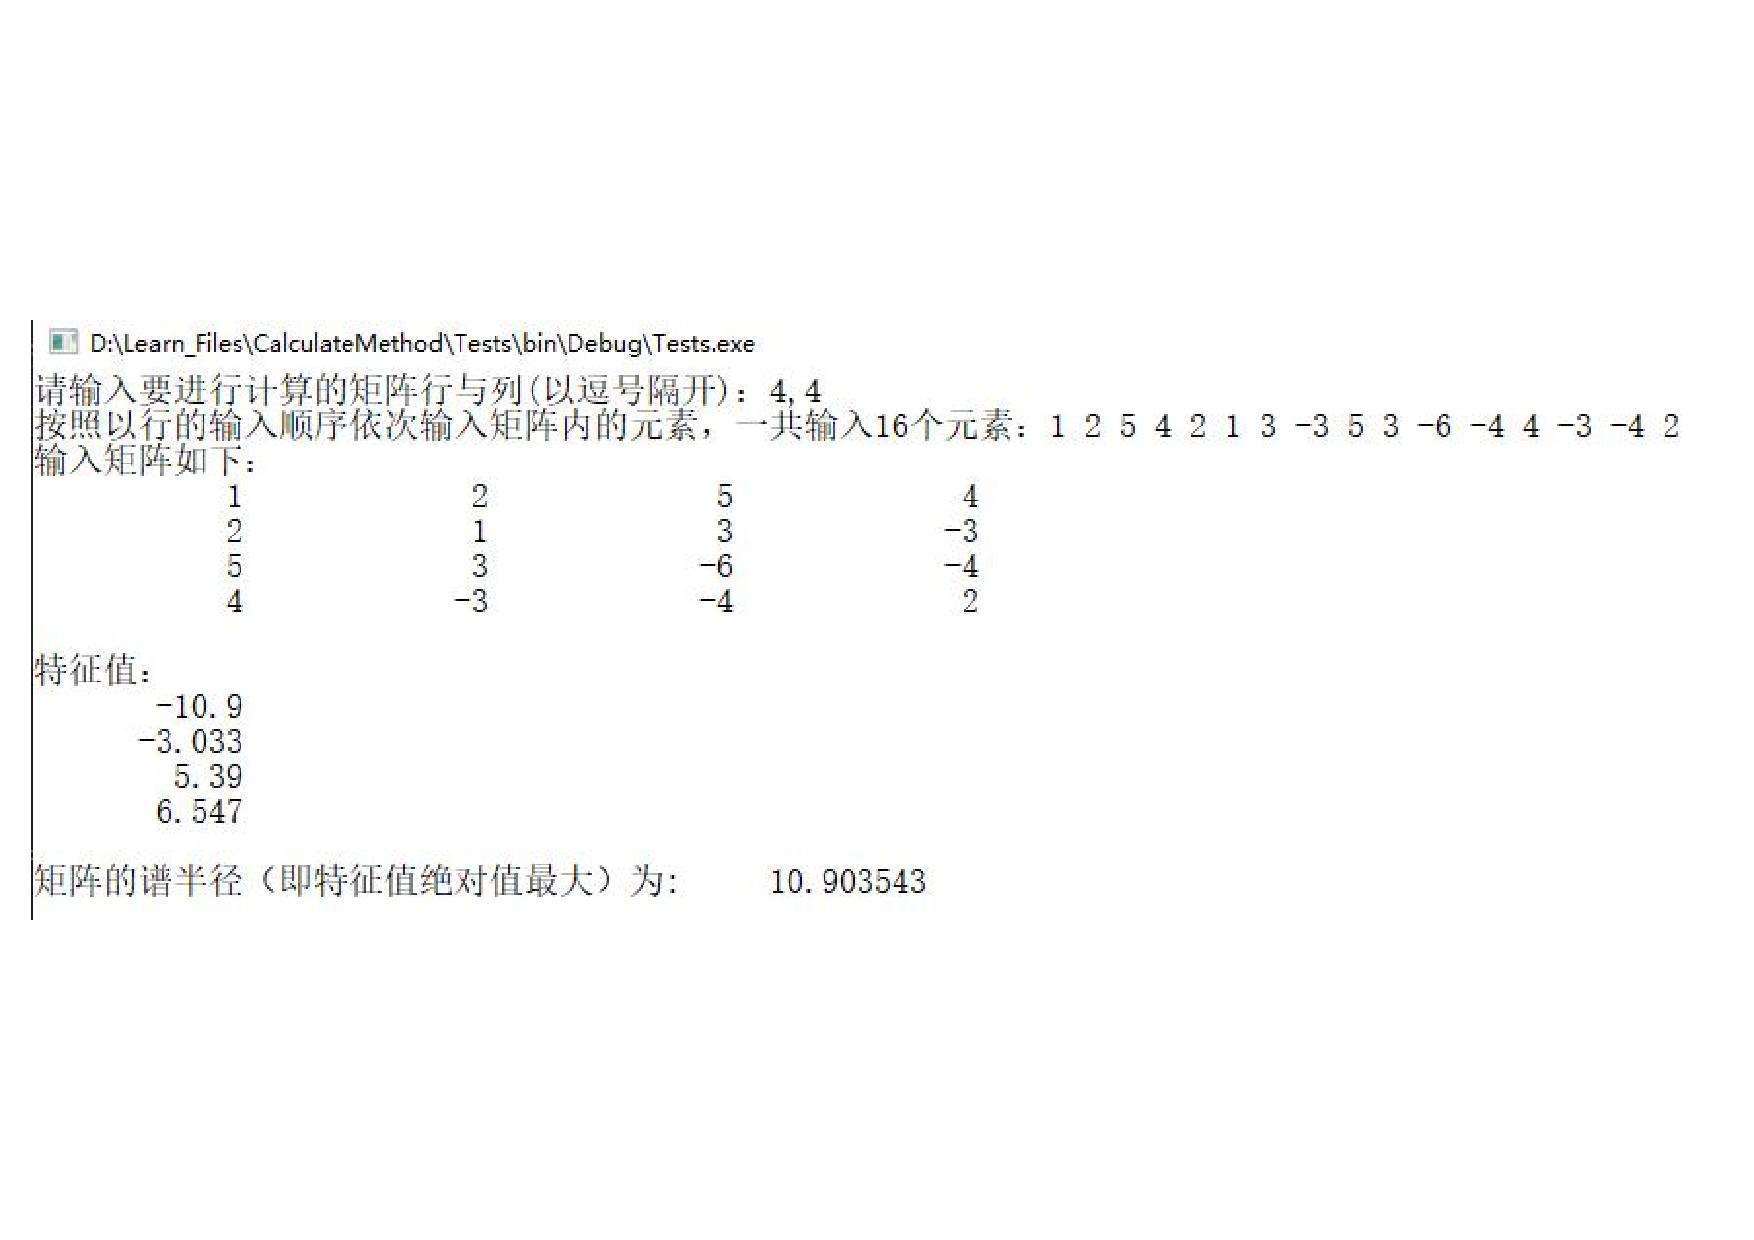
\includegraphics[width=0.6\textwidth]{result.pdf}
\caption{sample} \label{fig:sample}
\end{figure}


\begin{lstlisting}[language={c},
        numbers=left,
        numberstyle=\tiny\monaco,
        basicstyle=\footnotesize\monaco]
#include<stdio.h>
#include<stdlib.h>
#include <math.h>
#include <stdbool.h>

//定义一个结构体,用来表示一个二维的矩阵
typedef struct
{
	int row;
	int column;
	double *data;//用来存放矩阵的元素
}Matrix;

/************************************************************************
函数功能:初始化一个矩阵
输入:要初始化的矩阵matrix、矩阵的行row、矩阵的列column
输出:初始化成功:true;初始化失败:false
************************************************************************/
bool InitMatrix(Matrix *matrix, int row, int column)
{
	int matrix_size = row*column*sizeof(double);
	if (matrix_size <= 0)
		return false;
	matrix->data = (double*)malloc(matrix_size);//给矩阵分配空间
	if (matrix->data)
	{
		matrix->row = row;
		matrix->column = column;
		return true;
	}
	else
	{
		matrix->row = 0;
		matrix->column = 0;
		return false;
	}
}

/************************************************************************
函数功能:打印出一个矩阵
输入:一个矩阵matrix
输出:无
************************************************************************/
void PrintMatrix(Matrix *matrix)
{
	int matrix_num = matrix->row*matrix->column;
	for (int i = 0; i < matrix_num; i++)
	{
		printf("%12.4g  ", matrix->data[i]);
		if ((i + 1) % (matrix->column) == 0)
			printf("\n");
	}
	printf("\n");
}

/************************************************************************
函数功能:获取一个矩阵的大小
输入:一个矩阵matrix
输出:矩阵的大小size
************************************************************************/
int GetMatrixSize(Matrix *matrix)
{
	return matrix->row*matrix->column;
}

/************************************************************************
函数功能:清零,使矩阵每个元素为0
输入:需要清零的矩阵matrix
输出:无
************************************************************************/
void SetMatrixZeros(Matrix *matrix)
{
	int matrix_num = GetMatrixSize(matrix);
	for (int i = 0; i < matrix_num; i++)
		matrix->data[i] = 0;
}

/************************************************************************
函数功能:判断一个矩阵是否为空
输入:一个矩阵matrix
输出:为空则true,否则为false
************************************************************************/
bool IsNullMatrix(Matrix *matrix)
{
	int matrix_num =GetMatrixSize(matrix);
	if ((matrix_num <= 0) || (matrix->data == NULL))
		return true;
	else
		return false;
}

/************************************************************************
函数功能:释放掉一个矩阵
输入:一个矩阵matrix
输出:无
************************************************************************/
void DestroyMatrix(Matrix *matrix)
{
	if (!IsNullMatrix(matrix))
	{
		matrix->data = NULL;
		matrix->row = 0;
		matrix->column = 0;
		free(matrix->data);
	}
}

/************************************************************************
函数功能:计算一个矩阵的2范数,即求模
输入:一个矩阵matrix
输出:所求的范数结果norm2_ans
************************************************************************/
double MatrixNorm2(Matrix *matrix)
{
	double norm2_ans = 0.0;
	int matrix_num = GetMatrixSize(matrix);
	for (int i = 0; i < matrix_num; i++)
		norm2_ans+=(matrix->data[i]) * (matrix->data[i]);
	norm2_ans = (double)sqrt(norm2_ans);
	return norm2_ans;
}

/************************************************************************
函数功能:把一个矩阵复制
输入:需要进行复制的矩阵matrix_A,复制得到的一个矩阵matrix_B
输出:无
************************************************************************/
void CopyMatrix(Matrix *matrix_A, Matrix *matrix_B)
{
	if (matrix_B->row != matrix_A->row)
		matrix_B->row = matrix_A->row;
	if (matrix_B->column != matrix_A->column)
		matrix_B->column = matrix_A->column;
	int size_A = GetMatrixSize(matrix_A);
	for (int i = 0; i < size_A; i++)
		matrix_B->data[i] = matrix_A->data[i];
}

/************************************************************************
函数功能:对一个方阵A进行QR分解
输入:需要分解的矩阵A、分解后的正交矩阵Q和上三角矩阵R
输出:无
************************************************************************/
void QR(Matrix *A, Matrix *Q, Matrix *R)
{
	Matrix col_A, col_Q;
	InitMatrix(&col_A, A->row, 1);
	SetMatrixZeros(&col_A); //用来存A的每一列
	InitMatrix(&col_Q, A->row, 1);
	SetMatrixZeros(&col_Q);  //用来存Q的每一列

	if (A->row != A->column)
		printf("A is not a square matrix!");

	int A_size = GetMatrixSize(A);
	int Q_size = GetMatrixSize(Q);
	int R_size = GetMatrixSize(R);

	if (Q_size != A_size)
	{
		DestroyMatrix(Q);
		InitMatrix(Q, A->row, A->column);
		SetMatrixZeros(Q);
	}
	else
	{
		Q->row = A->row;
		Q->column = A->column;
		SetMatrixZeros(Q);
	}

	if (R_size != A_size)
	{
		DestroyMatrix(R);
		InitMatrix(R, A->row, A->column);
		SetMatrixZeros(R);
	}
	else
	{
		R->row = A->row;
		R->column = R->column;
		SetMatrixZeros(R);
	}

	//施密特正交化
	for (int j = 0; j < A->column; j++)
	{
		for (int i = 0; i < A->column; i++)//把A的第j列存入col_A中
		{
			col_A.data[i] = A->data[i * A->column + j];
			col_Q.data[i] = A->data[i * A->column + j];
		}
		for (int k = 0; k < j; k++)//计算第j列以前
		{
			R->data[k * R->column + j] = 0;
			for (int i1 = 0; i1 < col_A.row; i1++)
			{//R=Q'A(Q'即Q的转置) 即Q的第k列和A的第j列做内积
				R->data[k * R->column + j] += col_A.data[i1] * Q->data[i1 * Q->column + k];//Q的第k列
			}
			for (int i2 = 0; i2 < A->column; i2++)
			{
				col_Q.data[i2] -= R->data[k * R->column + j] * Q->data[i2 * Q->column + k];
			}
		}

		double temp = MatrixNorm2(&col_Q);
		R->data[j * R->column + j] = temp;
		for (int i3 = 0; i3 < Q->column; i3++)
		{
			//单位化Q
			Q->data[i3 * Q->column + j] = col_Q.data[i3] / temp;
		}
	}

	DestroyMatrix(&col_A);
	DestroyMatrix(&col_Q);
}

/************************************************************************
函数功能:给特征值排序,当flag=1时,则升序,当flag=0,则降序
输入:需要排序的序列eValue,升序还是降序的选择flag
输出:排序成功则返回true,否则返回false
************************************************************************/
bool SortEigenValues(Matrix *eValue, int flag)
{
	int size = GetMatrixSize(eValue);

	for (int i = 0; i < size - 1; i++)
	{
		int k = i;
		for (int j = i + 1; j < size; j++)
		{
			if (flag == 1)
			{
				if (eValue->data[k] > eValue->data[j])
				{
					k = j;
				}
			}
			else if (flag == 0)
			{
				if (eValue->data[k] < eValue->data[j])
				{
					k = j;
				}
			}
			else
				return false;
		}
		if (k != i)
		{
			double temp;
			temp = eValue->data[i];
			eValue->data[i] = eValue->data[k];
			eValue->data[k] = temp;
		}
	}
	return true;
}

/************************************************************************
函数功能:计算两个矩阵相乘C=A*B
输入:用来存计算结果的矩阵C、需要进行乘法计算的两个矩阵A和B
输出:计算成功则输出true,失败则false
************************************************************************/
bool MatrixMulMatrix(Matrix *C, Matrix *A, Matrix *B)
{
	if ((IsNullMatrix(A)) || (IsNullMatrix(B)))
		return false;

	int A_col = A->column;
	int B_row = B->row;
	InitMatrix(C, A->row, B->column);
	SetMatrixZeros(C);

	if (A_col != B_row)
	{
		printf("A_col!=B_row!");
		return false;
	}

	for (int i = 0; i < A->row; i++)
	{
		for (int j = 0; j < B->column; j++)
		{
			for (int k = 0; k < A->column; k++)
				C->data[i*C->row + j] += A->data[i*A->row + k] * B->data[k*B->column + j];
		}
	}

	return true;
}

int main()
{
	const unsigned NUM = 50; //最大迭代次数,让数据更准确
	Matrix mymatrix,temp,temp_Q,temp_R, eValue;
	int row,col;
	while (1)
	{
		printf("请输入要进行计算的矩阵行与列(以逗号隔开):");
		scanf("%d,%d", &row, &col);

		InitMatrix(&mymatrix, row, col);
		InitMatrix(&temp, row, col);
		SetMatrixZeros(&temp);
		SetMatrixZeros(&mymatrix);

		int num = row*col;
		printf("按照以行的输入顺序依次输入矩阵内的元素,一共输入%d个元素:", num);
		int data;
		for (int i = 0; i < num; i++)
		{
			scanf("%d", &data);
			mymatrix.data[i] = data;
		}
		printf("输入矩阵如下:\n");
		PrintMatrix(&mymatrix);

		CopyMatrix(&mymatrix, &temp);

		InitMatrix(&temp_Q, mymatrix.row, mymatrix.column);
		InitMatrix(&temp_R, mymatrix.row, mymatrix.column);
		InitMatrix(&eValue, mymatrix.row, 1);

		//使用QR分解求矩阵特征值
		for (int k = 0; k < NUM; ++k)
		{
			QR(&temp, &temp_Q, &temp_R);
			MatrixMulMatrix(&temp, &temp_R, &temp_Q);//R*Q
		}

		float result[temp.column];
		//获取特征值,将之存储于eValue
		for (int k = 0; k < temp.column; ++k)
		{
			eValue.data[k] = temp.data[k * temp.column + k];
			result[k] = fabs(temp.data[k * temp.column + k]);
		}

		SortEigenValues(&eValue, 1);//给特征值排序,1为升序,0为降序
		printf("特征值:\n");
		PrintMatrix(&eValue);

		float maxn = -1;
        for (int k = 0; k < temp.column; ++k)
		{
		    if (result[k] > maxn)
                maxn = result[k];
		}
		printf("矩阵的谱半径(即特征值绝对值最大)为:     %lf\n\n", maxn);

		DestroyMatrix(&eValue);
		DestroyMatrix(&mymatrix);
		DestroyMatrix(&temp);
		DestroyMatrix(&temp_Q);
		DestroyMatrix(&temp_R);
	}
	return 0;
}


\end{lstlisting}


\subsection{总结}
经过这次文章的撰写,我学到了很多知识。首先,对于题目而言,我学到了矩阵的特征值的计算,以及之后得到矩阵的谱半径,这让我又回忆起来线性代数的知识。其次,通过写文章,我对矩阵的谱半径有了更深的认识,而且,经过程序的编写,我又掌握了矩阵特征值的求法,这个看着简单,但实际写程序是很困难的。最后,我学习了怎么运用TeXworks软件写出漂亮的文章,它的排版和对数学公式的美化真的让我很喜欢。



%===参考文献===
%\addcontentsline{toc}{section}{参考文献}
%\bibliographystyle{abbrv}     %论文引用格式
%\bibliography{E:/studio/write/bibkit/wholebiblio}
                         
\begin{thebibliography}{99}
\bibitem{A19}
Author. {\em \color{red}Wiki}. \url{https://zh.wikipedia.org/wiki/%E8%B0%B1%E5%8D%8A%E5%BE%84}, 2019.

\bibitem{B19}
Author. {\em \color{blue}百度百科}. \url{https://baike.baidu.com/item/%E8%B0%B1%E5%8D%8A%E5%BE%84}, 2019.

\bibitem{C19}
Author. {\em CSDN}. \url{https://blog.csdn.net/qq_36417014/article/details/83901715}, 2019.

\bibitem{C19}
Author. {\em CSDN}. \url{https://blog.csdn.net/gsww404/article/details/78684278}, 2019.
\end{thebibliography}
\end{document}
%===结束===



History:
2019-10-23: 依据A19a创建;



